\documentclass[article]{ajs}\usepackage[]{graphicx}\usepackage[]{color}
%% maxwidth is the original width if it is less than linewidth
%% otherwise use linewidth (to make sure the graphics do not exceed the margin)
\makeatletter
\def\maxwidth{ %
  \ifdim\Gin@nat@width>\linewidth
    \linewidth
  \else
    \Gin@nat@width
  \fi
}
\makeatother

\definecolor{fgcolor}{rgb}{0.345, 0.345, 0.345}
\newcommand{\hlnum}[1]{\textcolor[rgb]{0.686,0.059,0.569}{#1}}%
\newcommand{\hlstr}[1]{\textcolor[rgb]{0.192,0.494,0.8}{#1}}%
\newcommand{\hlcom}[1]{\textcolor[rgb]{0.678,0.584,0.686}{\textit{#1}}}%
\newcommand{\hlopt}[1]{\textcolor[rgb]{0,0,0}{#1}}%
\newcommand{\hlstd}[1]{\textcolor[rgb]{0.345,0.345,0.345}{#1}}%
\newcommand{\hlkwa}[1]{\textcolor[rgb]{0.161,0.373,0.58}{\textbf{#1}}}%
\newcommand{\hlkwb}[1]{\textcolor[rgb]{0.69,0.353,0.396}{#1}}%
\newcommand{\hlkwc}[1]{\textcolor[rgb]{0.333,0.667,0.333}{#1}}%
\newcommand{\hlkwd}[1]{\textcolor[rgb]{0.737,0.353,0.396}{\textbf{#1}}}%

\usepackage{framed}
\makeatletter
\newenvironment{kframe}{%
 \def\at@end@of@kframe{}%
 \ifinner\ifhmode%
  \def\at@end@of@kframe{\end{minipage}}%
  \begin{minipage}{\columnwidth}%
 \fi\fi%
 \def\FrameCommand##1{\hskip\@totalleftmargin \hskip-\fboxsep
 \colorbox{shadecolor}{##1}\hskip-\fboxsep
     % There is no \\@totalrightmargin, so:
     \hskip-\linewidth \hskip-\@totalleftmargin \hskip\columnwidth}%
 \MakeFramed {\advance\hsize-\width
   \@totalleftmargin\z@ \linewidth\hsize
   \@setminipage}}%
 {\par\unskip\endMakeFramed%
 \at@end@of@kframe}
\makeatother

\definecolor{shadecolor}{rgb}{.97, .97, .97}
\definecolor{messagecolor}{rgb}{0, 0, 0}
\definecolor{warningcolor}{rgb}{1, 0, 1}
\definecolor{errorcolor}{rgb}{1, 0, 0}
\newenvironment{knitrout}{}{} % an empty environment to be redefined in TeX

\usepackage{alltt}

%%%%%%%%%%%%%%%%%%%%%%%%%%%%%%
%% declarations for jss.cls %%%%%%%%%%%%%%%%%%%%%%%%%%%%%%%%%%%%%%%%%%
%%%%%%%%%%%%%%%%%%%%%%%%%%%%%%


%% almost as usual
\author{Gregory B. Gloor\\The University\\ of Western Ontario \And 
        Jean M. Macklaim\\The University\\ of Western Ontario\And
        Michael Vu\\The University\\ of Western Ontario \And
         Andrew D. Fernandes\\YouKaryote Genomics\\ London, Canada  }
\title{Compositional uncertainty in high-throughput sequencing  data analysis should not be ignored}

%% for pretty printing and a nice hypersummary also set:
\Plainauthor{Gregory B. Gloor, Andrew D. Fernandes, Jean M. Macklaim, Michael Vu} %% comma-separated
\Plaintitle{Compositional uncertainty in high-throughput sequencing  data analysis should not be ignored} %% without formatting
\Shorttitle{Compositional Uncertainty in High-throughput Sequencing  Datasets} %% a short title (if necessary)

%% an abstract and keywords
\Abstract{
  The abstract of the article in English
  
}
\Keywords{Bayesian estimation, centred log-ratio, transcriptome, metagenome, 16S rRNA gene sequencing, ALDEx2, \proglang{R}}
\Plainkeywords{keywords, comma-separated, not capitalized, R} %% without formatting
%% at least one keyword must be supplied

%% publication information
%% NOTE: Typically, this can be left commented and will be filled out by the technical editor
%% \Volume{50}
%% \Issue{9}
%% \Month{June}
%% \Year{2012}
%% \Submitdate{2012-06-04}
%% \Acceptdate{2012-06-04}
%% \setcounter{page}{1}
\Pages{1--xx}

%% The address of (at least) one author should be given
%% in the following format:
\Address{
  Gregory B. Gloor\\
  Department of Biochemistry\\
  The University of Western Ontario\\
  London, Ontario, Canada\\
  E-mail: \email{ggloor@uwo.ca}\\
  URL: \url{http://www.academicbiography.uwo.ca/profile.php?&n=ggloor}
}
%% It is also possible to add a telephone and fax number
%% before the e-mail in the following format:
%% Telephone: +43/512/507-7103
%% Fax: +43/512/507-2851

%% for those who use Sweave please include the following line (with % symbols):
%% need no \usepackage{Sweave.sty}

%% end of declarations %%%%%%%%%%%%%%%%%%%%%%%%%%%%%%%%%%%%%%%%%%%%%%%
\IfFileExists{upquote.sty}{\usepackage{upquote}}{}
\begin{document}

%% include your article here, just as usual
%% Since this is an .Rnw document to be generated by knitr we need to generate some functions and load some data
%% We will not export this information



\section{Introduction}

High throughput sequencing studies, that   generate as outputs thousands to billions of sequence tags, are becoming the norm in the life sciences. That these experiments generate compositional data can be understood with two statements. First, the total number of sequence tags obtained in an experiment are of no importance. Second, the sequence tags are binned into features where the difference between features is exponential and best explained by ratios. These features can represent genes as in 16S rRNA gene sequencing, transcriptomics and metagenomics or single-nucleotide variant abundances after differential growth experiments. The experimentalist in these experiments is interested in knowing which features, if any, are differentially abundant between two or more distinct groups. Furthermore, all experiments of this type explicitly or implicitly examine sub-compositions. Finally, each individual experimental design is analyzed using different sets of underlying assumptions that are derived from historical dogma, despite having the same underlying data structure. Fernandes \citeyear{fernandes:2014} demonstrated that tools developed for one experimental design (e.g. RNA-Seq) do not translate well to other experimental designs (e.g. 16S RNA gene sequencing).

These data are necessarily sparse, and complex. There are often hundreds or thousands of features, and the expense of these experiments prevents the collection of sufficient sequence tags to ensure that all features are covered by at least one sequence tag. Thus, the treatment of features with zero counts is a pervasive problem when treating these data as compositions  \citep{lovell:2011}. It is assumed that features with zero counts across all samples are removed because they are uninformative. For the remainder where one approach is to  delete  features where one or more samples have zero counts  \citep{lovell:2011,lovell:2014}. This removes the problem of zero count features at the expense of   potentially excluding    the most important features from consideration. Another approach, is to replace the zero counts with an expected value calculated in some way. Several approaches with differing underlying assumptions are in use, and Mart\'{i}n-Fern\'{a}ndez \citeyear{fernandez:2014} suggested that a Bayesian-Laplace approach  to be the most reasonable. Regardless of the method used to treat zero count features, these analyses use maximum-likelihood approaches to determine feature abundance prior to analyses.

We have found that the variation due to sampling alone (technical variation) in compositional datasets derived from high-throughput sequencing is large and inversely related to the number of reads mapping to a fragment  \citep{fernandes:2013}. Ignoring this technical variation can lead to false positive inferences regarding differential abundance if the data are not treated as  compositions. We have found  that a two-step procedure  incorporating a Bayesian estimate of feature abundance along with analyses conducted after centred-log-ratio transformation markedly improves specificity with no loss of sensitivity, and that the increase in specificity derived almost entirely from the exclusion of low-count (including zero count) features  \citep{fernandes:2014}. 

Our paper  explores how the analyses differ when the value of zero is assigned using different approaches with, and without Bayesian estimation of the technical variation. Our initial work showed that a uniform prior added to all values was able to  encompass the estimated technical variation in a sparse dataset  \citep{fernandes:2013}. However, we observed that this approach slightly overestimated technical variation of low count and zero count features, suggesting that this approach had less than optimum power.

We will compare uniform priors that replace 0,  uniform priors added to all values, and the prior estimation methods from the zCompositions  package \citep{PalareaAlbaladejo201585} that produce non-uniform estimates of the actual zero value. We will examine a real differential growth experimental dataset for which an objective standard of truth is known. We argue that these results are generalizable across other datasets including RNA-seq datasets and 16S rRNA gene sequencing experiments. 

\section{Statement of the problem}

\vskip-0.25cm 
High throughput sequencing is a technology that delivers thousands to millions of reads that correspond uniquely to genes or other features in a genome, or to bins that represent sequence variants. Figure \ref{fig:design}A shows several different study designs that are common in the literature. Regardless of design a very large number of molecules, shown in the orange box in Figure \ref{fig:design}A are randomly sampled to produce a library that is then sequenced. The sequencing instrument delivers a much smaller random sample of the actual input and the act of sequencing converts the data from unconstrained to constrained proportional data because the instrument delivers a fixed number of sequence reads. This hard upper bound means that all such analyses generate compositional data regardless of the actual study design. In general, these experiments aim to ask the question, "what gene or feature has a different abundance between groups A and B?"

\begin{figure}[!ht]
\centerline{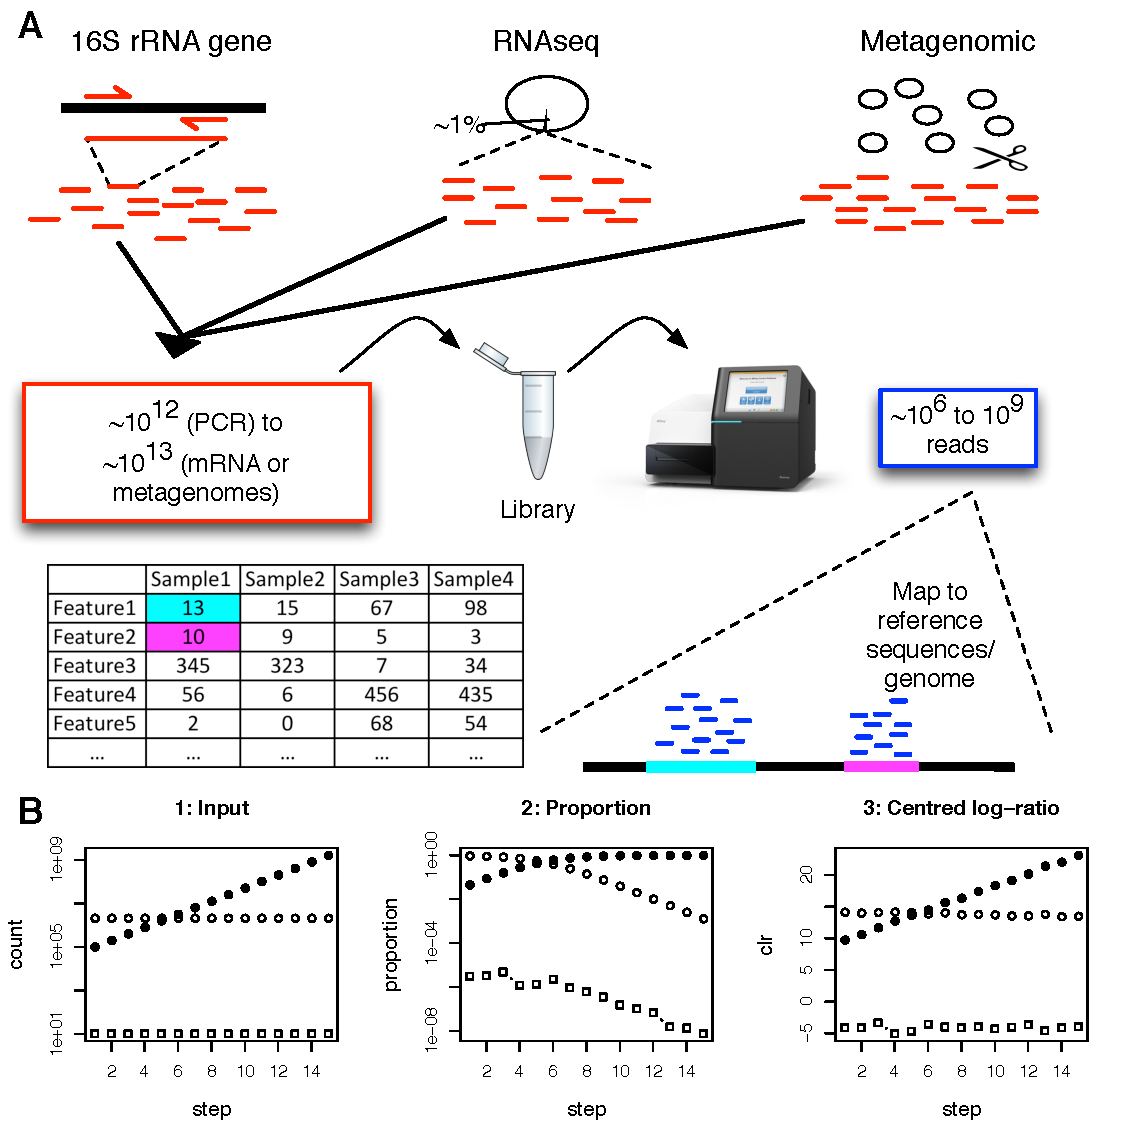
\includegraphics[width=4.6in]{fig_1.pdf}}
\vspace{3mm} \caption{High-throughput sequencing affects the shape of the data. Panel A illustrates the workflow by which high throughput sequencing samples the DNA or RNA from an environment. There are many more molecules that are sampled than can be incorporated into the library, or that can be sequenced on the instrument. The capacity of the instrument itself determines the number of reads observed. The orange box shows the number of molecules in typical initial samples, and the blue box shows the maximum number of reads that are obtained from the instrument. These reads are assigned to features such as genes or operational taxonomic units or other bins, and a table of the reads per feature is output. Panel B illustrates how the data is distorted during the process. The input DNA or RNA usually has no fixed sum and is randomly sampled sequentially   during the library preparation and sequencing steps. The output from the  instrument is compositional because the instrument can deliver only a fixed upper limit of reads, regardless of the number of molecules in the input. Panel B.1 shows the number of reads in the input tube for 15 steps where the open square and circular features are held at a constant number and the black feature is increasing in abundance by 2-fold each step. Panel B.2 shows the output in proportions (or ppm) after random sampling to a constant sum, as occurs on the sequencer. Panel B.3 shows the shape of the data following centre log-ratio transformation. Note that panels B.1 and B.2 have the y axis on a logarithmic scale, and that the natural scale for centred log-ratio data is logarithmic.}
\label{fig:design}
\end{figure}

Figure \ref{fig:design}B shows how sequencing distorts the data. Many processes examined by high throughput sequencing can be thought of as linear compositional processes. Consider a mixture of many distinctive molecules in vector $x=[x_1, x_2, ... x_n]$ over time or space increments $i$. For each increment we can determine the abundance of each molecule using Equation \ref{eq:process}:

\begin{equation}\label{eq:process}x_i = x_0 \times 2^{(\lambda  i)}\end{equation}

where $\lambda$ is the incremental rate. If $\lambda = 0$ for all but one of  the members of vector $x$ and $\lambda = 1$ for one member, then one member will double in abundance at each increment and all remaining members will be unchanged. Figure \ref{fig:design}B.1 shows such a thought experiment where the values are plotted as counts of molecules.  Producing and sequencing a library generates a set of counts per gene that are scaled by the maximum number of reads delivered by the machine. In other words, the counts for gene $x_i$ are per-gene probabilities $p_i$ and are formally equivalent to a random multivariate Poisson sample of the original group of DNA molecules. We model this process by sampling from the Dirichlet distribution according to Equation \ref{eq:dirichlet}:

\begin{equation}\label{eq:dirichlet} [p_1, p_2, ...p_n] \sim \mathrm{Dirichlet}[x_1, x_2, ... x_n].\end{equation}

A single Dirichlet instance generates a single Bayesian estimate of the underlying posterior probabilities for each feature, and multiple samples generate a full posterior distribution \citep{Holmes:2012,La-Rosa:2012,fernandes:2013}. Figure and panel \ref{fig:design}B.2 shows the posterior values for a single Dirichlet instance from the counts in Panel \ref{fig:design}B.1. Here we can see that the  constant sum constraint resulting from the finite read limit of the  instrument severely distorts the underlying shape of the data.  Figure \ref{fig:design}B.3 demonstrates that applying the standard centred log-ratio transform of Aitchison \citeyear{Aitchison:1986} to the vector of probabilities $p$ in Panel \ref{fig:design}B.1 

\begin{equation}\label{eq:clr}clr(p) = [log_2\frac{p_1}{g(p)},log_2\frac{p_2}{g(p)}, ... log_2\frac{p_n}{g(p)} ] \end{equation}

 reconstitutes the essential shape of the data, with the actual data points  now showing some variability because of random sampling. In  equation \ref{eq:clr}, $g(p)$ denotes the geometric mean of the vector $p$. This transformation is convenient because it reconstitutes the essential shape of the original data, and because there is a one to one mapping between the values in the original and in the transformed dataset. Furthermore, this transformation can easily interpreted for the experimentalist because it is simply a ratio between the abundance of a gene or feature in the sample and the average abundance of all genes or features in the sample. Of particular note is that $g(p)$ cannot be calculated when 0 values are present, and it is the influence of different means of estimating  0 values that are the primary focus of this report.  
 


\subsection{Data from high-throughput sequencing is highly variable}
Data from high throughput sequencing experiments are often thought of as point estimates despite being random samples of the input molecules, and despite several experiments showing that sequencing the same DNA library will produce somewhat different count tables at the same sequencing depth \citep{Marioni:2008,Bottomly:2011,Gierlinski:2015aa}.  Figure \ref{fig:qq} shows an example of this variability. Marioni et al. \citeyear{Marioni:2008} did an experiment where two aliquots  of the same RNA-seq library were run in duplicate, and the resulting reads  were mapped to the $>20000$ genes in the human genome. Replicate runs  did not return exactly the same number of reads per gene: for example, when the genes in  one replicate contained zero counts, the same genes in the other replicate  often had non-0 reads. This imprecision extends across the range of per-gene counts as shown for a few replicate read values in Figure \ref{fig:qq}. This imprecision is proportionally larger for small count values, and smaller for large count values. For example, the range of counts observed in replicate B when genes in replicate A contain one count span the range of 0-14 in this example: a difference of over 10-fold. By comparison, when genes in replicate A contain 64 counts the corresponding genes in replicate B span counts from 38-91: a difference of less than 50\%. See Figure 1 of Fernandes et al. \citeyear{fernandes:2013} for a demonstration that the proportional error does indeed span the entire range of expression values in this dataset.
%\subsubsection{Sampling from a Dirichlet distribution estimates this variability}
%\vskip-0.25cm

%%%%$ Dirichlet subsampling Figure
\begin{figure}[!ht]
\begin{center}
\begin{knitrout}
\definecolor{shadecolor}{rgb}{0.969, 0.969, 0.969}\color{fgcolor}
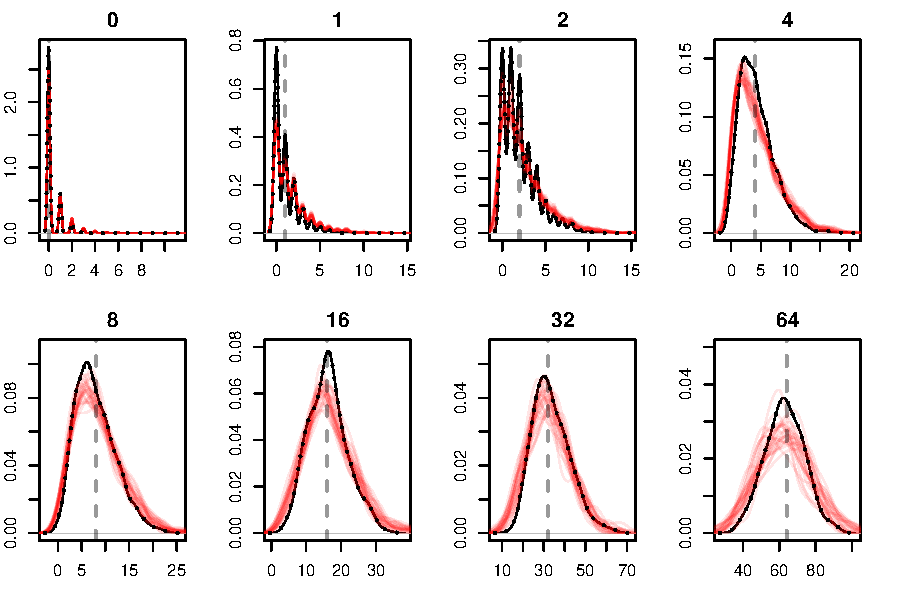
\includegraphics[width=\maxwidth]{figure/unnamed-chunk-1-1} 

\end{knitrout}
\caption{Technical replicate variation, and density plots of the estimation of that variation for an RNA-seq experiment. The black dotted lines show the density of the technical variation of features from one replicate of an RNA-seq dataset when compared to another as a function of the counts in the first replicate. The  count value of the first replicate  is give above each plot, and the location of this value is shown as the dotted grey vertical line. The red lines show density plots  of the inferred technical generated through 25 random instances drawn from  a Dirichlet distribution. Data are from the Marioni et al. \citeyear{Marioni:2008} dataset.}
\label{fig:qq}
\end{center}
\end{figure}

The imprecision can be modelled by sampling instances from a Dirichlet distibution  \citep{fernandes:2013,fernandes:2014} as in Equation \ref{eq:dirichlet}. Figure \ref{fig:qq} shows quantile-quantile plots comparing the distribution of true technical variation to the distribution of the estimated technical variation obtained  by drawing instances from the Dirichlet distribution. That is for a vector of counts $x$, $x_{Dir} = \mathrm{Dirichlet}[x] \times \sum x$. Sampling multiple Dirichlet instances thus returns a distribution of the posterior probabilities of each feature in the vector $x$, and conserves probability. These plots show that  the Dirichlet instances slightly over-estimate the tails of the distributions, although these conclusions need to be tempered by the lack of datapoint for technical replicates containing double-digit counts. We conclude that drawing Dirichlet instances is an acceptable method to model posterior probabilities in these datasets. 


\subsection{False positive results because of unaccounted variation}
\vskip-0.25cm 

One problem when analyzing such data is that the available datasets -- whether derived from 16S rRNA gene sequencing, transcriptomics, or other experiments -- are exploratory and so generally lack a standard of truth. This makes it difficult to develop and test tools without modelling a dataset. While modelled datasets have some allure because the parameters can be closely controlled,  we prefer to examine the behaviour of different approaches in real biological datasets because they often have unanticipated error and less predictable behaviour than modelled datasets.  

McMurrough et al. \citeyear{mcmurrough:2014} generated a selective growth dataset, hereafter called the `selex' dataset, for which a standard of truth for many variables is known, and that can be inferred for many others. This dataset compares the growth of a set of 1600 sequence variants in the I-LtrI endonuclease under two conditions. The first condition is a non-restrictive condition where the growth of all variants is unconstrained. The second condition is restrictive for growth, unless the I-LtrI endonuclease is active and can cleave and inactivate the gene encoding \emph{Ccdb}, a DNA gyrase toxin. The gyrase toxin is dose-dependent so cleavage of a fraction of the plasmids containing the gene  confers slower growth \citep{Smith:2006aa}, and under the conditions of the assay, the toxin would be bacteriostatic if no cleavage occurred. Thus in this experimental design the difference between inactive variants between the two conditions would be one of dilution alone, and \emph{no variant should become less abundant during the experiment}. Variants that cleave the toxin gene would confer a growth advantage, and would become more abundant over the time of the assay. Furthermore, McMurrough et al. \citeyear{mcmurrough:2014} showed that the \emph{in vitro} enzymatic activity of the endonuclease is strongly correlated with the output of the selective growth experiment.

The abundance of each variant in the mixture can be modelled by Equation \ref{eq:process}. At time zero if each variant is contained in vector $n_0=[n_1, n_2, n_3 ... n_{1600}]$, over time increments, the change in abundance in the non-selected growth conditions can be modelled with $\lambda = 1$ and the variation in $\lambda$ being small. The experimental conditions allowed for approximately 16 doublings, or time increments. Therefore at the last increment of the non-selected time series, we anticipate that the initial relationships between the abundances of each of the 1600 variants will be essentially unchanged. In contrast, the selected variants are under strongly differential selection. Here the most active variants will have $\lambda \approx 1$, that is, these variants grow at the same rate in the selected and unselected conditions. The least active variants will have $\lambda = 0$, that is, these variants will not change in actual abundance during selection, but will become relatively less abundant when compared to their active counterparts. Inactive variants are known to be by far the most prevalent in the samples.  Intermediate positive values of $\lambda$ are expected, and no negative values are expected. Finally, it is possible for individual samples to demonstrate differences in apparent $\lambda$ under selection. This can occur if a variant is partially active, and cleaves different proportions of  the toxin genes in a particular cell by chance. This  event is heritable and so would allow  cells carrying the same variant to grow at slightly different rates. Thus, the sample in which this occurred  would have an apparent increase in $\lambda$ for that variant in that sample.


%%%%$ zPatterns plot
\begin{figure}[!ht]
\begin{center}
\begin{knitrout}
\definecolor{shadecolor}{rgb}{0.969, 0.969, 0.969}\color{fgcolor}
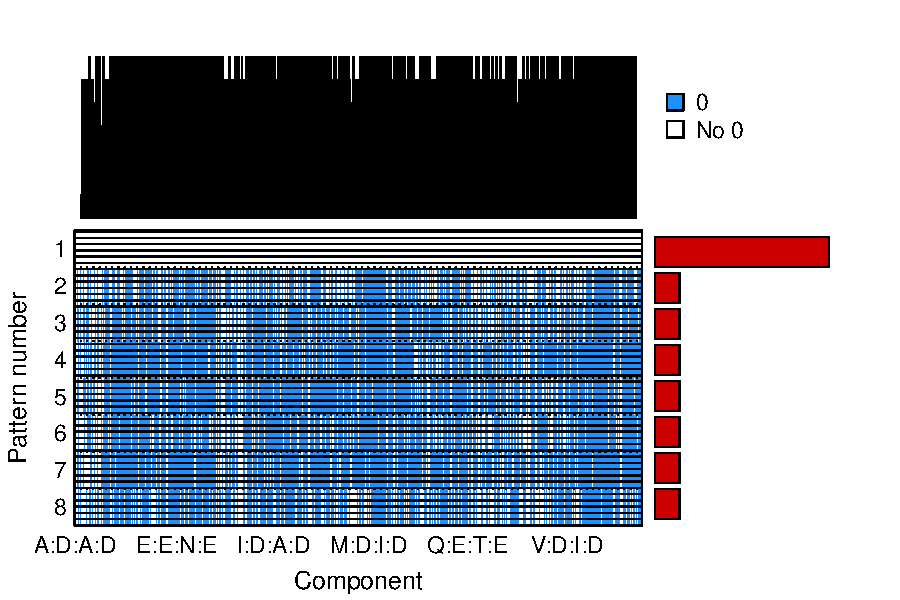
\includegraphics[width=\maxwidth]{figure/unnamed-chunk-2-1} 

\end{knitrout}
\caption{Characteristics of the McMurrough et al. \citeyear{mcmurrough:2014} dataset summarized by the zCompositions package. The top panel shows that all parts contain 0 values, and the bottom panel shows that there are 8 patterns in the data. Seven of the samples contain no 0 values, these are the control samples grown in the absence of selection. The samples derived from the selective growth display individual seven different patterns for 0 values likely due to random sampling.}
\label{fig:zPatterns}
\end{center}
\end{figure}

The question we wish to address with this dataset is: can we identify from the growth experiment alone which variants are likely to be active? Active variants will have had a maximum of 16 cell doublings becoming much more abundant, inactive variants will stay at the same abundance and variants with partial activity will become only somewhat more abundant. In addition, we wanted to know the effect on our inference of the different approaches to estimating the zero values. We  first examined the dataset using a biplot to show the relationship between the samples and the variants. 

%%%%$ CZM biplot Figure
\begin{figure}[!ht]
\centerline{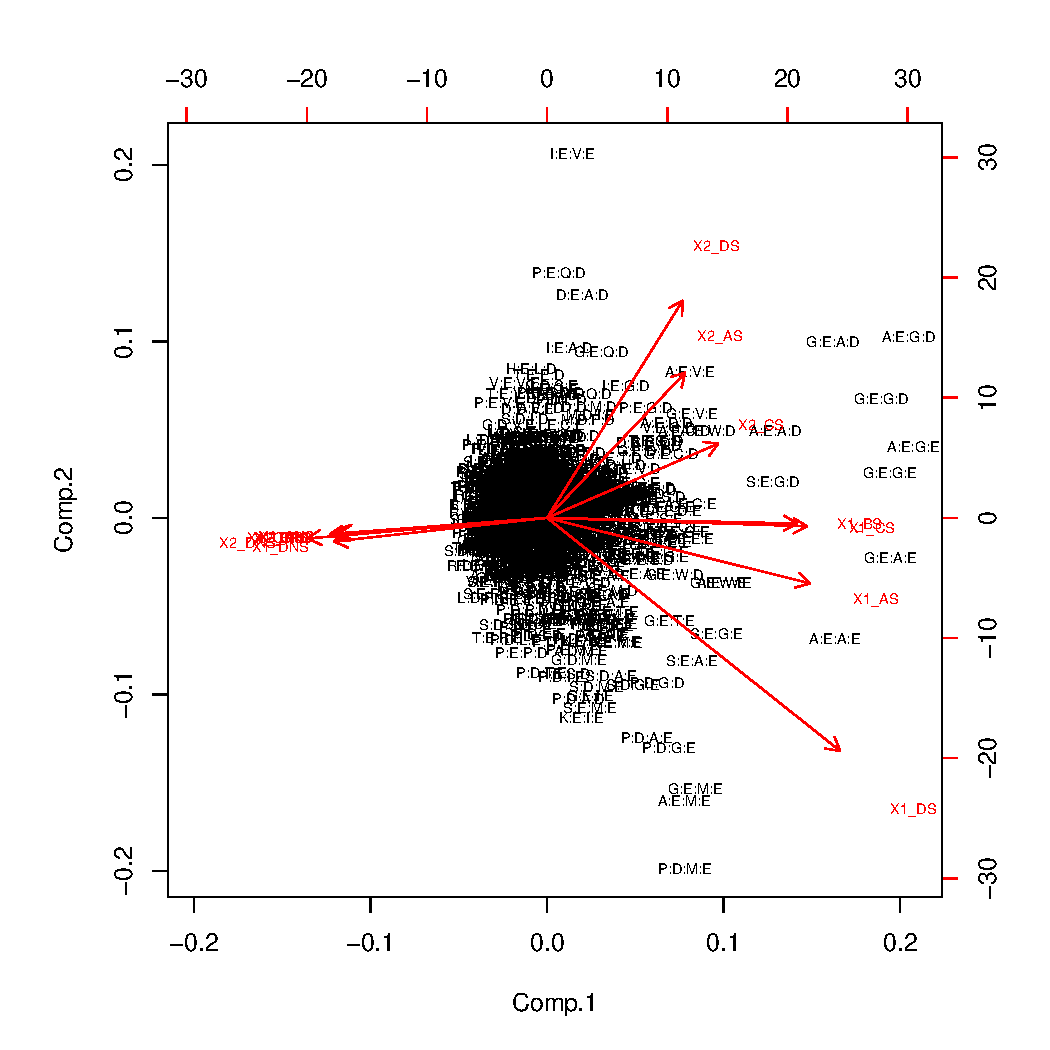
\includegraphics[width=5in]{/Users/ggloor/Documents/0_CoDa/0_2015/biplot_CZM.pdf}}
\vspace{3mm} \caption{Biplot showing the relationship between samples and variables in the selex dataset. Zero values were adjusted using the count zero multiplicative approach using the zCompositions \proglang{R} package, and the biplot was generated using the compositions \proglang{R} package. Samples ending with `NS' are the control non-selected growth samples and samples ending in `S'are from the selected growth samples.  The vast majority  of the variables cluster around the centre of the dataset. The red arrows to the left show that the 7 non-selected replicates are very similar, and the selected replicates on the right exhibit some variability. The differences between samples are driven by variation in a small number of variables.  In this dataset, component 1 explains 52.4\% of the variability and component 2 explains 10.4\%.}
\label{fig:biplot}
\end{figure}

Figure \ref{fig:zPatterns} shows the density and distributions of 0 values in this dataset as summarized by the zCompositions \proglang{R} package \citep{PalareaAlbaladejo201585}.  We can see that this dataset will be very challenging to analyze because the control samples do not contain any 0 values, but most of the variants in the experimental samples contain 0 values in several samples. This high density of 0 values comes about because the number of sequence reads was insufficient, and not because we expected a 0 value in any of the variants. Thus, we must impute the most likely value of 0 in each sample before analysis. 

A compositional biplot generated with the compositions \proglang{R} package \citep{vandenBoogaart2008320} following zero replacement using the CZM approach from the zCompositions \proglang{R} package \citep{PalareaAlbaladejo201585} is shown in Figure \ref{fig:biplot}. The first two components of this biplot explained 52.4\% and 10.4\% of the variance in the data, indicating that this is a good summary of the data. The selected and non-selected samples separate clearly on the first component, and this separation is driven largely by the abundance of the variants on the right side, such as A:E:G:E, G:E:G:E, G:E:G:E, etc,  which McMurrough et al. \citeyear{mcmurrough:2014} demonstrated to be the highly active variants. However, it is difficult to quantitate the magnitude of the abundance change of the variants from this analysis. This figure also shows that the  non-selected samples, which cluster on the left side, are essentially redundant since the links between them are exceedingly short. The selected samples on the right side are much more diverse, and some of the links from the origin are nearly orthogonal. The differences between the samples is largely on component 2, and is driven by the abundance of a small number of variants that also exhibit variation from the bulk on component 2. Inspection of the data finds that this diversity is driven by only a few variables such as I:E:V:E, P:D:M:E, A:E:M:E etc, and that these variables separate the X1 and X2 sample sets: interestingly, these sets are from identical experiments performed with different batches of the same cell type. Examination of the underlying count table shows that these variants are indeed  different in abundance between the X1 and X2 sets. For example the I:E:V:E variable has 17933 reads in sample X2\_DS but has zero reads in sample X1\_DS. This is an example of a single stochastic event that conferred a growth advantage to this variant in this sample. It is important to note that this large stochastic variation has important consequences when examining  datasets because such variation is not unusual in real biological datasets.


\subsubsection{Not accounting for sampling results in many false positive identifications}
\vskip-0.25cm

The selex dataset is unique because we have a validated truth for some of the features that differentiate the conditions \citep{mcmurrough:2014}. In this dataset we have unambiguously biochemically identified variants that are active and those that are not. Based on this prior information, we expect that approximately 60 variants would exhibit substantial activity in this assay, and so substantial deviation from this number would indicate many false positive results.

One approach that is widely used in the literature is to reduce the values from the count table to proportions or normalized counts through Maximum Likelihood approaches, then to conduct univariate statistical tests for each variant, and (sometimes) to correct for multiple testing (see for example the 16S rRNA analysis methods in Hsiao \citeyear{Hsiao:2013}). These approaches often treat zero values as actual zeros,  making no adjustments. Applying this simple method using an unpaired Wilcoxon test, and applying the Benjamini-Hochberg correction \citep{benjamini:1995} to the resulting P values reveals that 1593 of 1600 variants are identified as having a differential abundance between the selected and non-selected conditions with an adjusted P value cutoff of 0.05. This is clearly at odds with the known biology of the underlying dataset. 

A potentially more rigorous, yet still simple approach is to adjust the zero values in this dataset using one of the available methods that are implemented in the zCompositions \proglang{R} package \citep{PalareaAlbaladejo201585} and then to treat the data as compositions by applying Equation \ref{eq:clr} before performing univariate statistical tests. Recall from Figure \ref{fig:design} that this transformation recapitulates the essential shape of the data, and there is a one to one mapping of variant counts to centred log-ratio values. The range of values for zero replacement by different methods are given in the Prior column of Table \ref{tab:selex}. Interestingly, three of these zero correction methods returned values greater than 1 for some of the zero values, this likely was a result of the very large difference between the selected and non-selected count values in the two groups. In addition, we applied two other approaches to deal with zero values. The first, labeled uniform replacement, replaces all zero values with 0.5 but does not adjust other values in the dataset. This is akin to adding a pseudo count to zero values. The second labelled uniform prior, applies a uniform prior adjustment to \emph{all values} in the  dataset. For this we use the minimally informative Jeffrey's prior of 0.5. The Comp 1 and Comp 2 columns in Table \ref{tab:selex} show the percentage variation explained by a clr compositional biplot using each of these zero adjustments in the first two principle components. Only the biplot that used the square-root Bayesian multiplicative  method appears to result in a transformation that explains substantially less of the variation in the dataset. 

\begin{table}[!htdp]
\caption{Numbers of distinguishing features identified in the selective growth experiment observed with different approaches to assign prior expectations to zero count features.}
\begin{center}
\begin{tabular}{lccccr}
Prior assignment  & Prior & Comp 1 & Comp 2 & Point & Dir\\ \hline
Count zero  & 0.325452 - 0.325910 & 0.524 & 0.104  & 874 & 91\\
Geometric Bayesian  & 0.061279 - 4.890273 &0.504 & 0.108 & 355 & 82\\
Square root  & 0.006854 - 3.102299 & 0.452 & 0.118 & 1008 & DNR\\
Bayes-Laplace & 0.030497 - 4.883747 & 0.480 & 0.108 & 435 & 133\\
Uniform replacement & 0.5 & 0.556 & 0.098 & 958 & 74\\
Uniform Prior  & 0.5 & 0.528 & 0.102 & 868 & 84\\

\end{tabular}
\end{center}
\label{tab:selex}
\end{table}%


The utility of these zero replacement approaches to detect univariate differences in this experiment was tested closing the  vectors after prior assignment, applying the centred log-ratio transform to each sample and then subjecting the features to  unpaired Wilcoxon tests. Again P values were adjusted using the Benjamini-Hochberg method and an adjusted P value of 0.05 was used as the threshold for significance. Table \ref{tab:selex}-Point shows the results of this approach. Here we see that all of the methods substantially improve upon the naive approach, with between one-quarter and two-thirds of the variables being identified as differential. In this dataset, the  square root Bayesian multiplicative method provides the largest number of positive identifications, and the Geometric Bayesian multiplicative correction provides the smallest number of positive identifications, although no method is able to strongly distinguish the known small number of true positives from a much larger number of false positives.

\subsubsection{Accounting for sampling reduces false positive identifications}

One substantial  shortcoming of these approaches is that the inherent technical variation in the dataset is not taken into account. It is becoming an accepted practice to account for the sampling using  Dirichlet multinomial mixture models, where each sample is represented by a vector of probabilities, rather than point estimates \citep{Holmes:2012}. For example, Ding \citeyear{Ding:2014aa} recently used this approach to  partition microbiomes into different community states in a robust manner. This approach thus generates a Bayesian posterior estimate of the probabilities associated with each count prior to analysis.

This approach was tested by generating 128 Dir instances of the selex dataset using Equation \ref{eq:dir} with a uniform prior of 0.5, and then conducted per-variant Wilcoxon tests on each instance. The mean Benjamini-Hochberg adjusted P value for each variant was tabulated, and again the cutoff used was an adjusted P value of 0.5. Surprisingly, this approach, which takes into account the inferred technical variation, again resulted in 1593 of the 1600 variants as being differentially abundant between the selected and non-selected groups. This is more than the 868 variants detected when variation was not taken into account but the centred log-ratio transform was applied, and equivalent to the naive method accounting for neither variation nor the compositional nature of the data. Thus, simple averaging across inferred the technical variates is not sufficient to screen out false positive variants in this dataset. 

Finally, we combined the Bayesian posterior estimated from 128 Dirichlet instances of the data and the centred log-ratio transformation of the posterior and used this as the input to significance tests.  This method is implemented in the ALDEx2 \proglang{R} package for the analysis of high throughput sequencing datasets \citep{fernandes:2013,fernandes:2014}, and is available at Bioconductor. 

As implemented, the ALDEx2 package uses the uniform zero replacement value of 0.5. One purpose of this investigation was to determine if using one of the more rigorous zero replacement models from the zCompositions package would increase our selectivity because, as shown in Table \ref{tab:selex}, these adjustments output non-uniform estimates of the underlying value of zero based on abundances of the same feature in different samples. 

We applied the same seven methods to adjust the value of zero in the selex dataset, and an overview of the results are shown in the Dir column of Table \ref{tab:selex}. We again used Wilcoxon tests on the two groups and corrected the resulting P values using the Benjamini-Hochberg approach. Significance was assumed if the mean adjusted P value across all 128 instances was less than 0.05.  In this analysis the substituted values of zero in the adjusted datasets serve as prior estimates of the range of values that zero could assume in each of the Dirichlet instances.  The square root Bayesian multiplicative approach was incompatible with generating Dirichlet instances because many of the prior values that replaced zero generated Dirichlet posterior estimates that were not distinguishable from zero. Modelling uniform priors indicated that this occurred when the prior for zero was less than approximately 0.05. The remaining six approaches were compatible with the approach, and resulted in substantially smaller numbers of variants being identified as significantly different between the selected and non-selected groups. In this analysis, the Geometric Bayesian multiplicative, uniform replacement and uniform prior approaches were approximately similar, the count zero multiplicative  approaches was nearly as selective, and the Bayes-Laplace approach was least selective. 

\begin{figure}[!ht]
\centerline{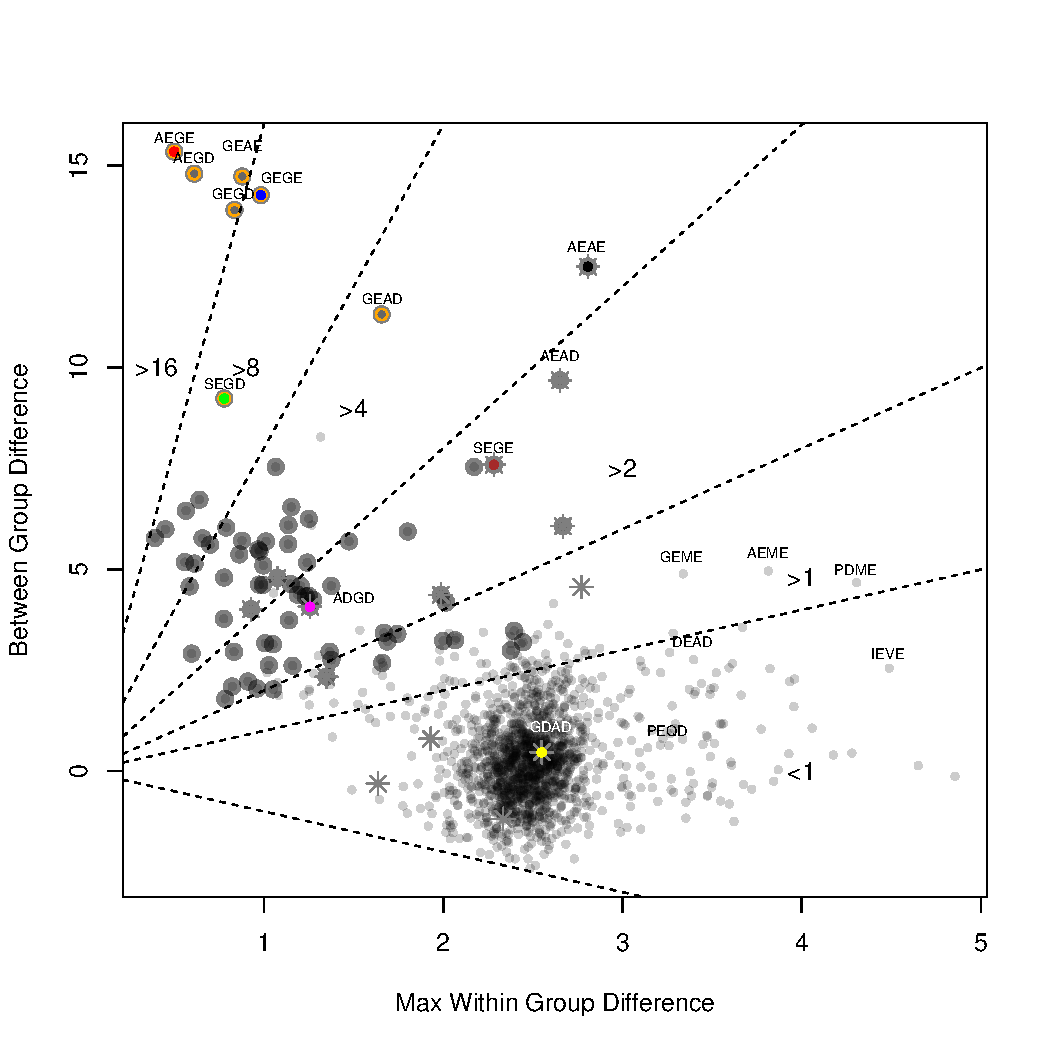
\includegraphics[width=4.6in]{/Users/ggloor/Documents/0_CoDa/0_2015/all_tested.pdf}}
\vspace{3mm} \caption{Variance-variance plot showing the median maximum centred log-ratio scaled difference within each group plotted vs. median between group difference for each variant. Dotted lines represent the approximate location of effect sizes, which is calculated as the median between to within group difference. Variants are coloured if their activity was validated \emph{in vitro}, have a star if they failed to grow reliably in individual culture \emph{in vitro}. Variants that exhibit a significant increase in abundance using the Wilcoxon test with a mean Benjamini-Hochberg adjusted P value of $> 0.05$ are shown as large grey dots. The analysis was done with a uniform prior of 0.5 applied to the dataset. Also shown are the six variants that were outliers on component 2 of the clr biplot in Figure \ref{fig:biplot}}
\label{fig:vv}
\end{figure}


Figure \ref{fig:vv} shows a variance-variance plot of the output from  an analysis using the uniform prior replacement with a value of 0.5. Note that in this plot the vast majority of variants have an estimated between group difference of approximately zero, that only a small number have a positive between group difference, and no variants have a strong negative between group difference. This fits with the experimental design where variants could increase in abundance if the endonuclease was active, but not decrease in abundance if it was not. In this plot the variants with a mean Benjamini-Hochberg adjusted P value determined by an unpaired Wilcoxon test are indicated by the large grey dots. Variants that were tested for enzymatic activity \emph{in vitro} are indicated by coloured central dots. Variants that had near wild type enzymatic activity \emph{in vitro} are in the sector marked as $>8$. There were four variants that had partial enzymatic activity \emph{in vitro}. Many variants were tested for growth in pure culture. Variants AEAE, SEGE, ADGD and GDAD exhibited variable, partial growth under these conditions, with the GDAD variant exhibiting the weakest growth. Thus, there is a strong relationship between the observed results in this experiment, and the results observed \emph{in vitro}.


There is remarkable concordance between the data viewed in this way, and the same data viewed as a point estimate in the compositional biplot. The biplot shows that the most distinguishing variants between the selected and non-selected groups, i.e., the variants that drive the separation on principle component 1, are those in the upper left quadrant of Figure \ref{fig:vv}. In addition, the variants that drive the separation on principle component 2, are those that exhibit the largest within-condition difference. For example, the GEME, AEME, PDME, IEVE, PEQD, and DEAD variants that were strongly separated on component 2 on the biplot, are among those with the largest within group difference on the variance-variance plot.

% CZM 0.3254517 0.3259098
% BL 0.03049729 4.88374704
% GBM  0.06127945 4.89027346
% SQ 0.00685417 3.10229876
\begin{figure}[1ht]
\centerline{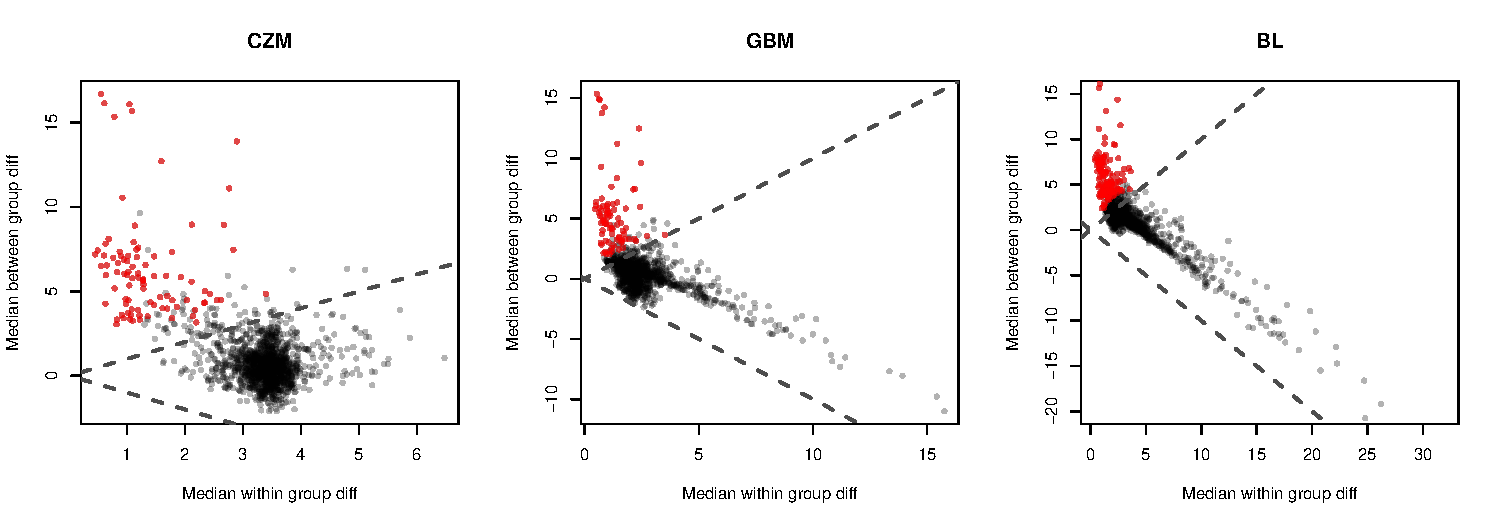
\includegraphics[width=5.5in]{/Users/ggloor/Documents/0_CoDa/0_2015/zero_replace.pdf}}
\vspace{3mm} \caption{Variance-variance  plots showing how the prior values for zero determined by the count zero multiplicative (CZM), geometric Bayesian multiplicative (GBM) and Bayes-Laplace (BL) methods alter the variation of the data. Red dots represent those that are called differential, black dots are not differential and the lines represent effect sizes of 1 and -1. The cutoff used was a Benjamini-Hochberg adjusted P value of 0.05 from an unpaired Wilcoxon test.  }
\label{fig:replace}
\end{figure}

Finally, we examined the effect of the different zero replacement methods on the shape of the variance-variance plot to determine why these different approaches deliver slightly different results after Dirichlet sampling log-ratio transformation. As shown in Figure \ref{fig:replace} all the prior estimation methods delivered similar differences between conditions for the true positive variants. These all exhibited an increase in abundance of about $2^{16}$ relative to their mean abundance in the unselected group. In particular, the CZM plot was remarkably similar  to the plot that used a uniform prior of 0.5, with the major difference between the two approaches being a slight broadening of the within-group difference. This is perhaps not surprising since the prior values of zero using this approach are non-uniform in a narrow range of near 0.325. In contrast the non-uniform prior values for zero count variants from both the GBM and BL ranged over much larger values. The vast majority of values were between zero and one, but the GBM method had an average of 197.4 zero replacements that were greater than one, and the BL had an average of 55 replacements that were greater than one. Examination of the variance-variance plots of these two approaches showed that between-group difference for many variants was not significant, but tended to be strongly negative. This result is incompatible with the known biology of the experiment, where no variant is expected to become less abundant than average in the selected dataset. Therefore, in this dataset, the geometric Bayesian multiplicative and the Bayes-Laplace substitution methods are distorting the underlying data. This distortion likely contributes to the greater number of variants identified as significantly different between the selected and non-selected groups.  

\section{Discussion}
\vskip-0.25cm 

High throughput sequencing datasets are  different from other types of datasets to which compositional approaches are often applied, but fall into the general class of `count compositional' data. However, it is useful to remember that high throughput sequencing datasets result from random sampling of a large number of DNA fragments, and that the act of sequencing these DNA fragments on the instrument results in data that has the constant sum constraint. The estimation of the true abundance of genes or features with low counts exhibits a very large proportional error.  

It is tempting to imagine that the large number of counts observed for a given sample, ranging from the thousands to billions, provides great precision in estimating the true values of the genes or OTUs (parts) being examined. This is an erroneous assumption because there are hundreds to thousands of parts in each sample, and many of the parts will be represented by zero reads in some samples. Thus, it is more useful to think of these data as \emph{one instance of the data observed from a single random sample}. When thinking about the data in this way, the reads per part in each sample can be represented as prior values for a Bayesian estimation of their posteriors. The  posterior distribution of the underlying abundance of each feature can be estimated by generating multiple instances of the data by sampling from a Dirichlet distribution. 

As noted above, these datasets are necessarily very sparse, but in many cases the sparsity is informative. For example, in 16S rRNA gene sequencing it is difficult to argue that a particular taxonomic group would \emph{never} be observed if we generated sufficient sequencing reads. As another example, gene expression is stochastic, and the number of transcripts for a given gene is observed not to be zero when large populations of cells are sampled, even if the gene in question is `not expressed' \citep{Munsky:2012aa}. 

The centred log-ratio approach is intrinsically attractive in a biological context for two reasons. First, it can be intuitively explained to biologists as being similar to quantitative PCR, a familiar technique where the ratio between the gene of interest and a gene assumed to be at a constant level is determined. The centred log-ratio approach merely extends this analogy to the ratio between the gene of interest and all other genes in the system. Second, biologists understand that many of the processes that they study, cell growth, enzyme kinetics, etc, are exponential processes. Less well understood is that the underlying data is not `set in stone' but actually represents a snapshot of what would have been observed had the experiment been done again.  

A common criticism of using log-ratio approaches when analyzing such sparse data is the problem of zero observed counts. Structural zeros, those features that contain zero in every sample, are always excluded, and do not cause problems. However, count zeros that occur in one condition but not the other are problematic because log-ratio transformations cannot be performed when the underlying data contains one or more features with a zero value \citep{Aitchison:1986}. Much work has been put into this problem because of the prevalence of features with values of zero are common in many kinds of datasets. Several approaches have been developed to determine the best point estimate of the actual underlying value of zero in these datasets \citep{pawlowsky2015modeling}, and they are implemented in zCompositons \proglang{R} package \citep{PalareaAlbaladejo201585}. Less work has been done modelling this in a Bayesian framework where the distribution of probable values for each variable are taken into account. 

Here we have examined the effect of using various approaches to estimating the value of zero on both point estimates and Bayesian distributions derived from Dirichlet multinomial sampling. We have found that point estimates, whether modelled as proportions or centre log-ratio transformed values,  cannot distinguish features that differ between conditions in a problematic dataset. We found that estimating the technical variation alone is also unsuitable. However, the combination of estimating technical variation and the centre log-ratio transformation provides a large increase in selectivity. We further observe that methods that  generate priors in a narrow range give outputs that closely mimic a dataset derived from a differential growth experiment, and that methods that generate priors with broad ranges generate posterior distributions that are different from the known underlying distribution.

The selex dataset is an extreme example of the type of data that is  analyzed by high throughput sequencing. It has a small number of features that exhibit a marked difference in abundance between conditions, and is very sparse. Other experimental designs will have much smaller difference in abundance of features. For example, in the case of  RNA-seq it is more common to examine differential abundance of a small number of genes that are themselves relatively rare in the cell, and from carefully controlled experiments where the total number of input molecules is similar between conditions. This would be akin to comparing steps 1 and 2 in Figure \ref{fig:design}B.1, where no gene or set of genes perturbs the system signfificantly. In this simple case, any approach would likely give reasonable answers. However, comparing gene expression between cells from different tissues, or gene expression in RNA from environmental samples, would introduce  extreme distortions in the underlying data and could give false positive and false negative results \citep{fernandes:2013,macklaim:2013,fernandes:2014}. In the case of 16S rRNA gene sequencing experiments, it is likely that many conditions would have wildly divergent underlying abundances because bacterial growth is an exponential process, and such samples are more difficult to analyze. 

\section*{Acknowledgements}
\vskip-0.25cm
This work was supported by a grant to Greg Gloor by the National Science and Engineering Research Council of Canada.  


Correspondence addresses of author(s) should be added at the end
of the manuscript. 



%\bibliographystyle{plainat}
\bibliography{bibdesk_refs}



\end{document}
